%%%%%%%%%%%%%%%%%%%%%%%%%%%%%%%%%%%%%%%%%
% Jacobs Landscape Poster
% LaTeX Template
% Version 1.0 (29/03/13)
%
% Created by:
% Computational Physics and Biophysics Group, Jacobs University
% https://teamwork.jacobs-university.de:8443/confluence/display/CoPandBiG/LaTeX+Poster
%
% Further modified by:
% Nathaniel Johnston (nathaniel@njohnston.ca)
%
% This template has been downloaded from:
% http://www.LaTeXTemplates.com
%
% License:
% CC BY-NC-SA 3.0 (http://creativecommons.org/licenses/by-nc-sa/3.0/)
%
%%%%%%%%%%%%%%%%%%%%%%%%%%%%%%%%%%%%%%%%%

%----------------------------------------------------------------------------------------
%   PACKAGES AND OTHER DOCUMENT CONFIGURATIONS
%----------------------------------------------------------------------------------------

\documentclass[final]{beamer}
\usepackage[utf8]{inputenc}
\usepackage[T1]{fontenc}
\usepackage[english]{babel}

\usepackage[scale=1.24]{beamerposter} % Use the beamerposter package for laying out the poster

\usetheme{confposter} % Use the confposter theme supplied with this template

\setbeamercolor{block title}{fg=ngreen,bg=white} % Colors of the block titles
\setbeamercolor{block body}{fg=black,bg=white} % Colors of the body of blocks
\setbeamercolor{block alerted title}{fg=white,bg=dblue!70} % Colors of the highlighted block titles
\setbeamercolor{block alerted body}{fg=black,bg=dblue!10} % Colors of the body of highlighted blocks
% Many more colors are available for use in beamerthemeconfposter.sty

%-----------------------------------------------------------
% Define the column widths and overall poster size
% To set effective sepwid, onecolwid and twocolwid values, first choose how many columns you want and how much separation you want between columns
% In this template, the separation width chosen is 0.024 of the paper width and a 4-column layout
% onecolwid should therefore be (1-(# of columns+1)*sepwid)/# of columns e.g. (1-(4+1)*0.024)/4 = 0.22
% Set twocolwid to be (2*onecolwid)+sepwid = 0.464
% Set threecolwid to be (3*onecolwid)+2*sepwid = 0.708

\newlength{\sepwid}
\newlength{\onecolwid}
\newlength{\twocolwid}
\newlength{\threecolwid}
\setlength{\paperwidth}{46.8in} % A0 width: 46.8in
\setlength{\paperheight}{33.1in} % A0 height: 33.1in
\setlength{\sepwid}{0.024\paperwidth} % Separation width (white space) between columns
\setlength{\onecolwid}{0.22\paperwidth} % Width of one column
\setlength{\twocolwid}{0.464\paperwidth} % Width of two columns
\setlength{\threecolwid}{0.708\paperwidth} % Width of three columns
\setlength{\topmargin}{-0.8in} % Reduce the top margin size
%-----------------------------------------------------------

\usepackage{graphicx}  % Required for including images

\usepackage{booktabs} % Top and bottom rules for tables

\usepackage[final]{listings}
%\usepackage{verbatimbox}
%\usepackage{fancyvrb}
\usepackage[nounderscore]{syntax}

\usepackage{xcolor}
%\definecolor{butter}{HTML}{FCE94F}
%\definecolor{butter}{HTML}{EDD400}
\definecolor{butter}{HTML}{C4A000}
%\definecolor{orange}{HTML}{FCAF3E}
%\definecolor{orange}{HTML}{F57900}
\definecolor{orange}{HTML}{CE5C00}
%\definecolor{chocolate}{HTML}{E9B96E}
%\definecolor{chocolate}{HTML}{C17D11}
\definecolor{chocolate}{HTML}{8F5902}
%\definecolor{chameleon}{HTML}{8AE234}
%\definecolor{chameleon}{HTML}{73D216}
\definecolor{chameleon}{HTML}{4E9A06}
%\definecolor{skyblue}{HTML}{729FCF}
%\definecolor{skyblue}{HTML}{3465A4}
\definecolor{skyblue}{HTML}{204A87}
%\definecolor{plum}{HTML}{AD7FA8}
%\definecolor{plum}{HTML}{75507B}
\definecolor{plum}{HTML}{5C3566}
%\definecolor{scarletred}{HTML}{EF2929}
%\definecolor{scarletred}{HTML}{CC0000}
\definecolor{scarletred}{HTML}{A40000}
%\definecolor{lightalu}{HTML}{EEEEEC}
%\definecolor{lightalu}{HTML}{D3D7CF}
\definecolor{lightalu}{HTML}{BABDB6}
%\definecolor{darkalu}{HTML}{888A85}
%\definecolor{darkalu}{HTML}{555753}
\definecolor{darkalu}{HTML}{2E3436}

\newcommand{\kwstyle}{}

\usepackage{listings}

\lstset{
%	backgroundcolor=\color{},
	basicstyle=\small\ttfamily\color{black},
%	breakatwhitespace=false,
	breaklines=true,
%	captionpos=b,
	commentstyle=\color{darkalu},
%	deletekeywords={...},
%	escapeinside={\%*}{*)},
%	extendedchars=true,
%	frame=single,
%	keepspaces=true,
	keywordstyle=\kwstyle,
	language=Caml,
%	morekeywords={*,...},
%	numbers=left,
%	numbersep=5pt,
%	numberstyle=\color{},
%	rulecolor=\color{},
%	showspaces=false,
%	showstringspaces=false,
%	showtabs=false,
%	stepnumber=2,
	stringstyle=\color{plum},
	tabsize=2,
%	title=\lstname,
	keywordstyle=[1]\kwstyle\color{chameleon},
	keywordstyle=[2]\kwstyle\color{scarletred},
	keywordstyle=[3]\kwstyle\color{skyblue},
	keywordstyle=[4]\kwstyle\color{butter},
	keywordstyle=[5]\kwstyle\color{skyblue},
	keywordstyle=[6]\kwstyle\color{skyblue},
	keywordstyle=[7]\kwstyle\color{chameleon},
	keywordstyle=[8]\kwstyle\color{butter},
	keywordstyle=[9]\kwstyle\color{butter},
	keywords=[1]{let,val,method,in,and,rec,private,virtual,constraint},
	keywords=[2]{type,open,class,module,exception,external},
	keywords=[3]{fun,function,functor,match,try,with},
	keywords=[4]{as,when,of},
	keywords=[5]{if,then,else},
	keywords=[6]{begin,end,object,struct,sig,for,while,do,done,to,downto},
	keywords=[7]{true,false},
	keywords=[8]{include,inherit,initializer},
	keywords=[9]{new,ref,mutable,lazy,assert,raise},
}

\lstset{literate=
	{0}{{{\kwstyle\color{plum}0}}}1 {0.}{{{\kwstyle\color{plum}0.}}}2
	{1}{{{\kwstyle\color{plum}1}}}1 {1.}{{{\kwstyle\color{plum}1.}}}2
	{2}{{{\kwstyle\color{plum}2}}}1 {2.}{{{\kwstyle\color{plum}2.}}}2
	{3}{{{\kwstyle\color{plum}3}}}1 {3.}{{{\kwstyle\color{plum}3.}}}2
	{4}{{{\kwstyle\color{plum}4}}}1 {4.}{{{\kwstyle\color{plum}4.}}}2
	{5}{{{\kwstyle\color{plum}5}}}1 {5.}{{{\kwstyle\color{plum}5.}}}2
	{6}{{{\kwstyle\color{plum}6}}}1 {6.}{{{\kwstyle\color{plum}6.}}}2
	{7}{{{\kwstyle\color{plum}7}}}1 {7.}{{{\kwstyle\color{plum}7.}}}2
	{8}{{{\kwstyle\color{plum}8}}}1 {8.}{{{\kwstyle\color{plum}8.}}}2
	{9}{{{\kwstyle\color{plum}9}}}1 {9.}{{{\kwstyle\color{plum}9.}}}2
	{->}{{{\kwstyle\color{chameleon}$\rightarrow$}}}2
}


%\lstset{basicstyle=\footnotesize\ttfamily,breaklines=true}
%\lstset{language=Caml}
%\lstset{
% literate=
%  {->}{$\rightarrow{}$}{1}
%  {<-}{$\leftarrow{}$}{1},
% morekeywords={open,module,implicit,struct,sig,end,val}
%}

%----------------------------------------------------------------------------------------
%   TITLE SECTION
%----------------------------------------------------------------------------------------

\title{Inuit: from printf to interactive user-interfaces} % Poster title

\author{Fr\'ed\'eric Bour} % Author(s)

\institute{OCL, University of Cambridge} % Institution(s)

%----------------------------------------------------------------------------------------

\begin{document}

\addtobeamertemplate{block end}{}{\vspace*{2ex}} % White space under blocks
\addtobeamertemplate{block alerted end}{}{\vspace*{2ex}} % White space under highlighted (alert) blocks

\setlength{\belowcaptionskip}{2ex} % White space under figures
\setlength\belowdisplayshortskip{2ex} % White space under equations

\begin{frame}[containsverbatim,t] % The whole poster is enclosed in one beamer frame

\begin{columns}[t] % The whole poster consists of three major columns, the second of which is split into two columns twice - the [t] option aligns each column's content to the top

\begin{column}{\sepwid}\end{column} % Empty spacer column

\begin{column}{\onecolwid} % The first column

%-------------------------------------------------------------------------------
%   FIRST COLUMN
%-------------------------------------------------------------------------------

\begin{block}{Introduction}

  As OCaml doesn't favor introspection, long-running processes risk turning into
  black boxes.

  Common solutions to observe internal state are printf-debugging/logging or
  relying on heavier GUI toolkits. The former is limited; the latter is harder
  to develop and has higher requirements.

  Inuit extends the printf approach and narrow the gap with GUI toolkits.

  It aims at exposing a model that is:

  \begin{itemize}
  \item easy to use for interactive monitoring, tracing, and configuration of
    services;
  \item good enough for simple text-based UI.
  \end{itemize}

\end{block}

\begin{alertblock}{Programming model}
  Inuit is a library to build and update a semi-structured text document.

  The central concept is the \textbf{region}. A region abstracts a range of
  characters and can contain sub-regions.  The following primitives can be
  applied:

  \begin{itemize}
    \item {\em append} inserts text;
    \item {\em clear} erases everything in the region;
    \item {\em sub} creates and returns a new sub-region.
  \end{itemize}

  From a root region and these primitives one can build and
  update a tree of textual regions.
\end{alertblock}

\begin{block}{Rendering the document}
Inuit keeps track of the document structure and turns the content into simple
{\em patches} -- a patch inserts, removes or replaces a range of text. Text
itself is not stored by Inuit.
A {\em backend} consumes the stream of patches.

This design makes it easy to switch between backends.  The default one
serializes patches to a channel, to be consumed by external processes.  No
dependency are introduced.
\end{block}

\end{column} % End of the first column

\begin{column}{\sepwid}\end{column} % Empty spacer column

\begin{column}{\twocolwid} % The second column

%------------------------------------------------

\begin{alertblock}{Region API}

\begin{lstlisting}
type 'flags t
(** Type of a region.
    'flags are associated to text content. They don't affect the document
    structure but allow to extend the text with backend specific information
    (styling, interactions, etc).  *)

val append : 'flags t -> 'flags list -> string -> unit
(** Add text to the right end of the region. *)

val clear : 'flags t -> unit
(** Erase the content, including sub-regions. *)

val sub : ?observer:'flags observer -> 'flags t -> 'flags t
(** Append a new sub-region.  Multiple calls to sub form a tree of regions.
    [observer] is a callback that allow to observe changes. *)

val make : unit -> 'flags t * 'flags patch socket
(** Creating a root region. It also returns the patch stream for the backend. *)
\end{lstlisting}

%\textbf{Cursors.} \lstinline|'flags| are necessary for composing rich text
%properties.  Inuit exposes a convenient \lstinline|'flags cursor| type.  It
%simply packs a region and a default set of flags.

\end{alertblock}


\begin{columns}[t,totalwidth=\twocolwid] % Split up the two columns wide column

\begin{column}{\onecolwid}\vspace{-.6in} % The first column within column 2 (column 2.1)

\begin{block}{Flexible deployment}

The only backend available today displays content in Emacs.  The UI is
presented in a buffer.  Communication is done with a custom sexp-based
protocol.

Different setups are supported:

\begin{description}
  \item[Commands] communicating over stdin/stdout.
  \item[Services] listening on a UNIX Domain Socket.
  \item[Remote display.] The protocol handles long latencies well.
    Applications can run transparently over a network connection such as SSH.
\end{description}
\end{block}

\begin{block}{Extended features}

Extra information is communicated via flags. They don't affect the
structure, just the interaction.  If a flag is not supported by a backend,
functionalities are degraded but the content remains available.

A reasonable set of flags is still being devised.   Current implementation
includes {\em clickable} and {\em editable} areas, {\em focus} management, and
{\em custom face} selection.

\end{block}

\end{column}

\begin{column}{\onecolwid}\vspace{-.6in} % The second column within column 2 (column 2.1)

\begin{block}{Simple trace}
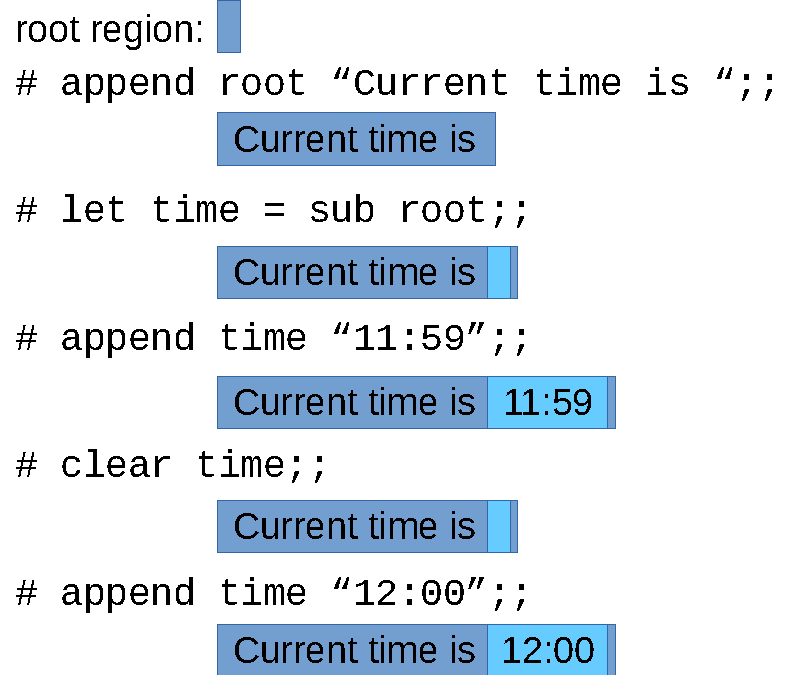
\includegraphics[width=0.8\onecolwid]{trace}
\end{block}

\begin{block}{Practical applications}
A few applications have been developed to validate the library.

Top-level integration, a replayable trace library, a frontend for interactive
fictions.  Introspection for Merlin (state monitoring, interactive logging).

Frontends for OCaml tools: {\em landmarks} and {\em spacetime} profilers and
{\em ocp-index} library browser.


%Some patterns ended up in a small library of generic widgets (treeview,
%editable-field, navigation history).
\end{block}

\end{column}

\end{columns}

\end{column} % End of the second column

\begin{column}{\sepwid}\end{column} % Empty spacer column

\begin{column}{\onecolwid} % The third column

\begin{block}{Rendering pipeline details}
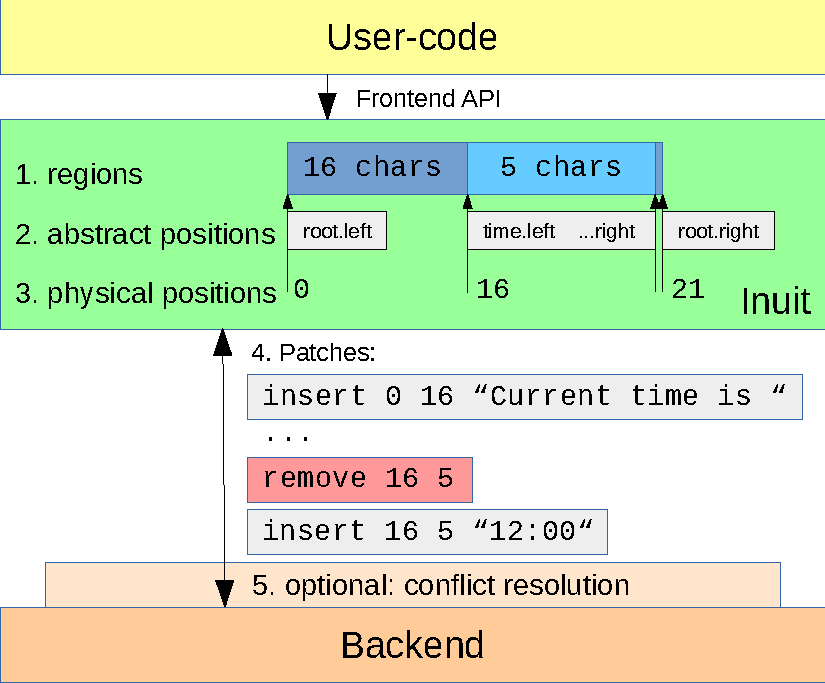
\includegraphics[width=\onecolwid]{pipeline}

Inuit exposes regions (1), forming a tree of nested positions (2).  Positions
can be mapped to physical offsets (3). User actions update this tree and are
turned into a stream of patches (4).

Since backend might executes asynchronously, an optional conflict resolution
pass can be applied (5).
\end{block}

\begin{block}{Future work}
A TTY backend is planned for development soon.  A NeoVim backend is being
considered too, but cleaning up the protocol specification and providing
stronger typing is a prerequisite.

Among possible applications for Inuit we would like to experiment hyper-linked
navigation in OCaml documentation.

\end{block}

\setbeamercolor{block alerted title}{fg=black,bg=norange} % Change the alert block title colors
\setbeamercolor{block alerted body}{fg=black,bg=white} % Change the alert block body colors

\begin{alertblock}{Implementation prototype}
The library is licensed under ISC license.

Development happens on github:
\begin{description}
  \item[Inuit library:]
    \href{https://github.com/let-def/inuit}{github.com/let-def/inuit}
  \item[Emacs backend:]
    \href{https://github.com/let-def/sturgeon}{github.com/let-def/sturgeon}

% LOGO
\begin{center}
\begin{tabular}{c}

\includegraphics[width=0.4\linewidth]{logo.png}
\end{tabular}
\end{center}

\end{description}

\end{alertblock}

\end{column} % End of the third column

\begin{column}{\sepwid}\end{column} % Empty spacer column

\end{columns}

\end{frame} % End of the enclosing frame

\end{document}
